\chapter{Classificatori multiclasse}
\paragraph{Tavola di contingenza.} La tavola di contingenza si ampia per i classificatori multiclasse semplicemente aggiungendo righe e colonne per ogni classe:
\begin{figure}[!h]
    \centering
    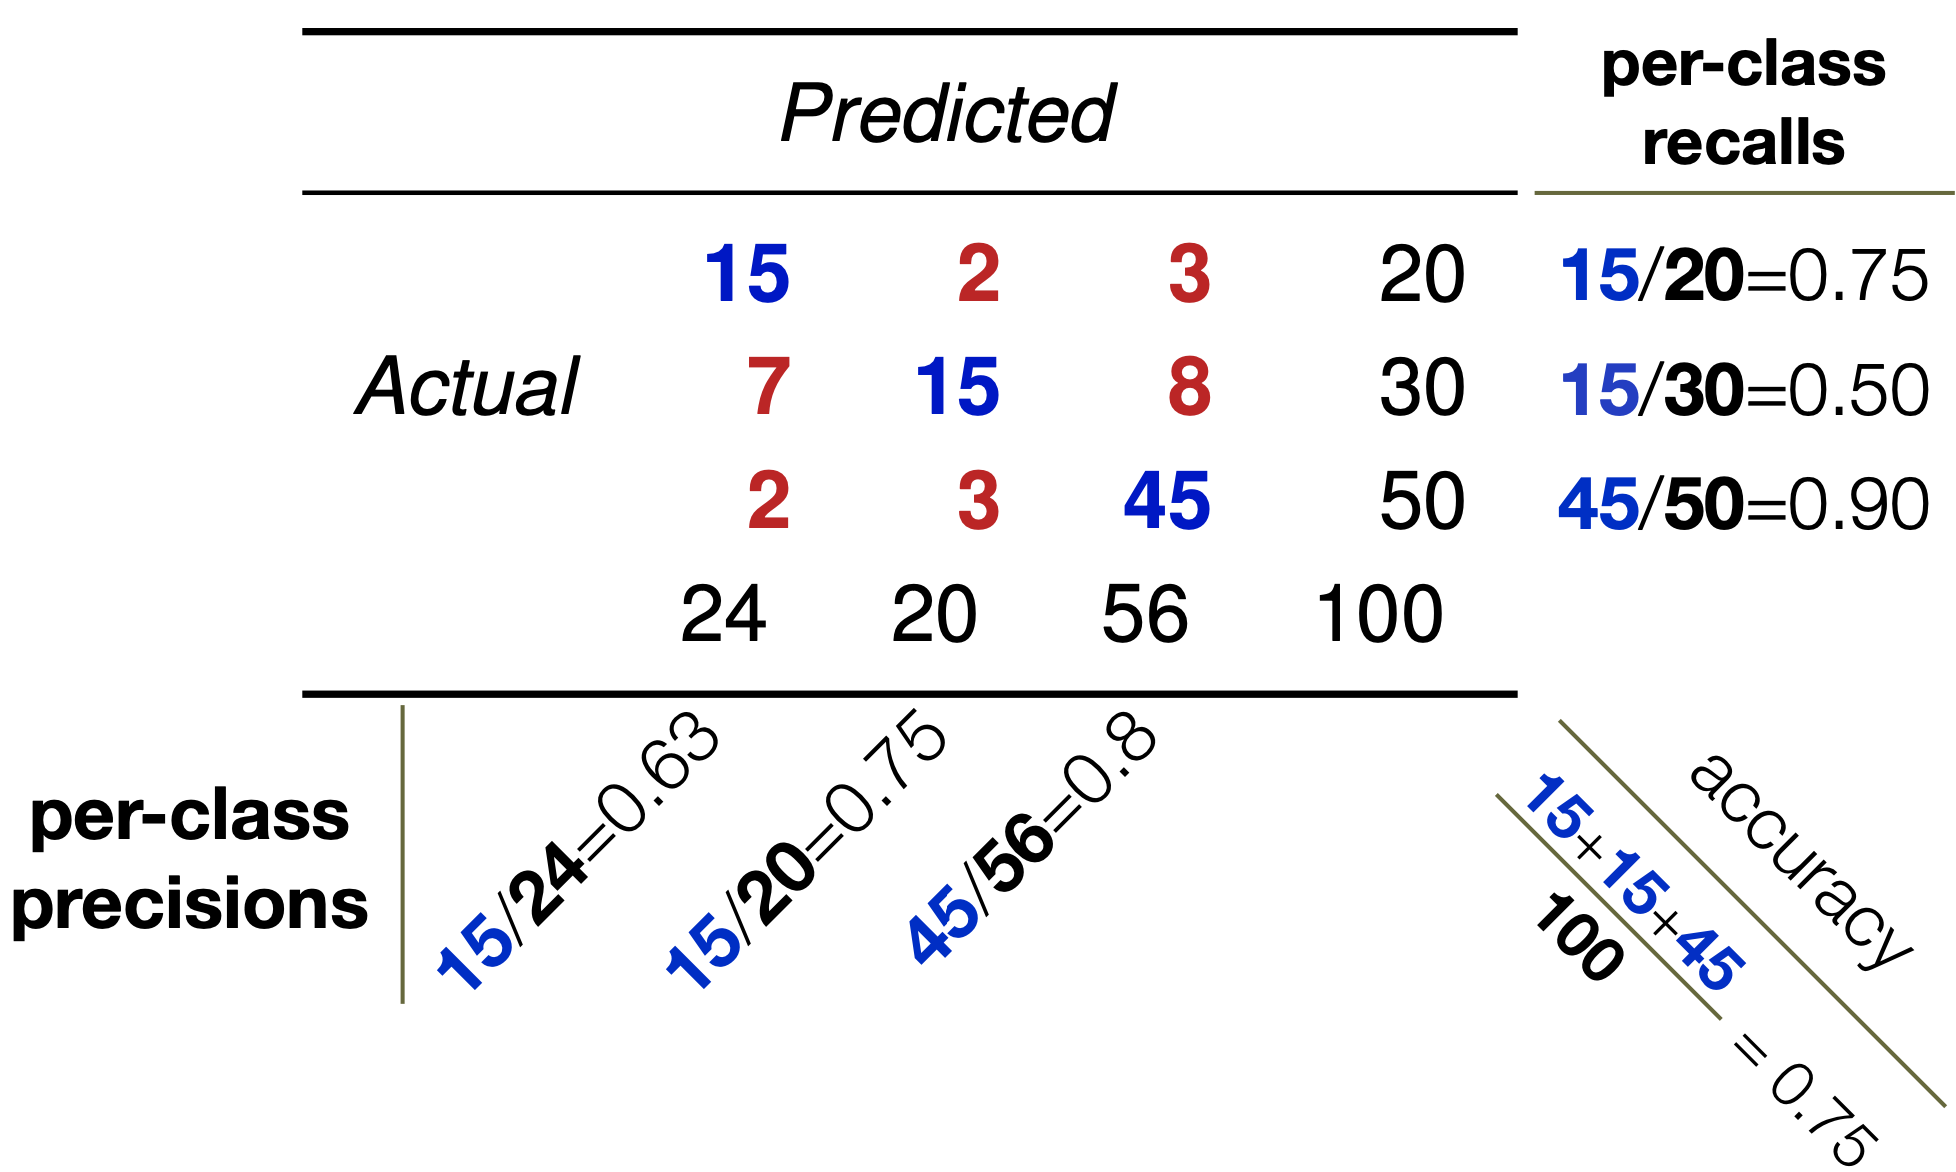
\includegraphics[scale=0.3]{images/multiContTab.png}
    \label{fig:enter-label}
\end{figure}

\section{Estendere classificatori da binari a multiclasse}
Ci sono varie tecniche per risolvere un problema multiclasse usando un classificatore binario, tra questi:
\begin{itemize}
    \item schemi \textbf{uno contro tutti}:
        \begin{itemize}
            \item apprendimento non ordinato,
            \item apprendimento ordinato.
        \end{itemize}
    \item schemi \textbf{uno contro uno}:
        \begin{itemize}
            \item simmetrico,
            \item asimmetrico.
        \end{itemize}
\end{itemize}
L'idea è trasformare il problema di apprendimento, cambiando le etichette del training set e trasformando il problema principale in un certo numeri di problemi binari. Acquisire poi un classificatore binario su questi dataset modificati e poi combinare questi classificatori in un'unica predizione alla fine del processo.

\newpage
\paragraph{Uno contro tutti (non ordinato)} Abbiamo un dataset definito su 3 classi e un certo numero di istanze. Per risolvere il problema, assumiamo di avere a disposizione un algoritmo di apprendimento $L:X^n\rightarrow (X\rightarrow \{-1,1\} )$, cioè un classificatore binario.
\begin{figure}[!h]
    \centering
    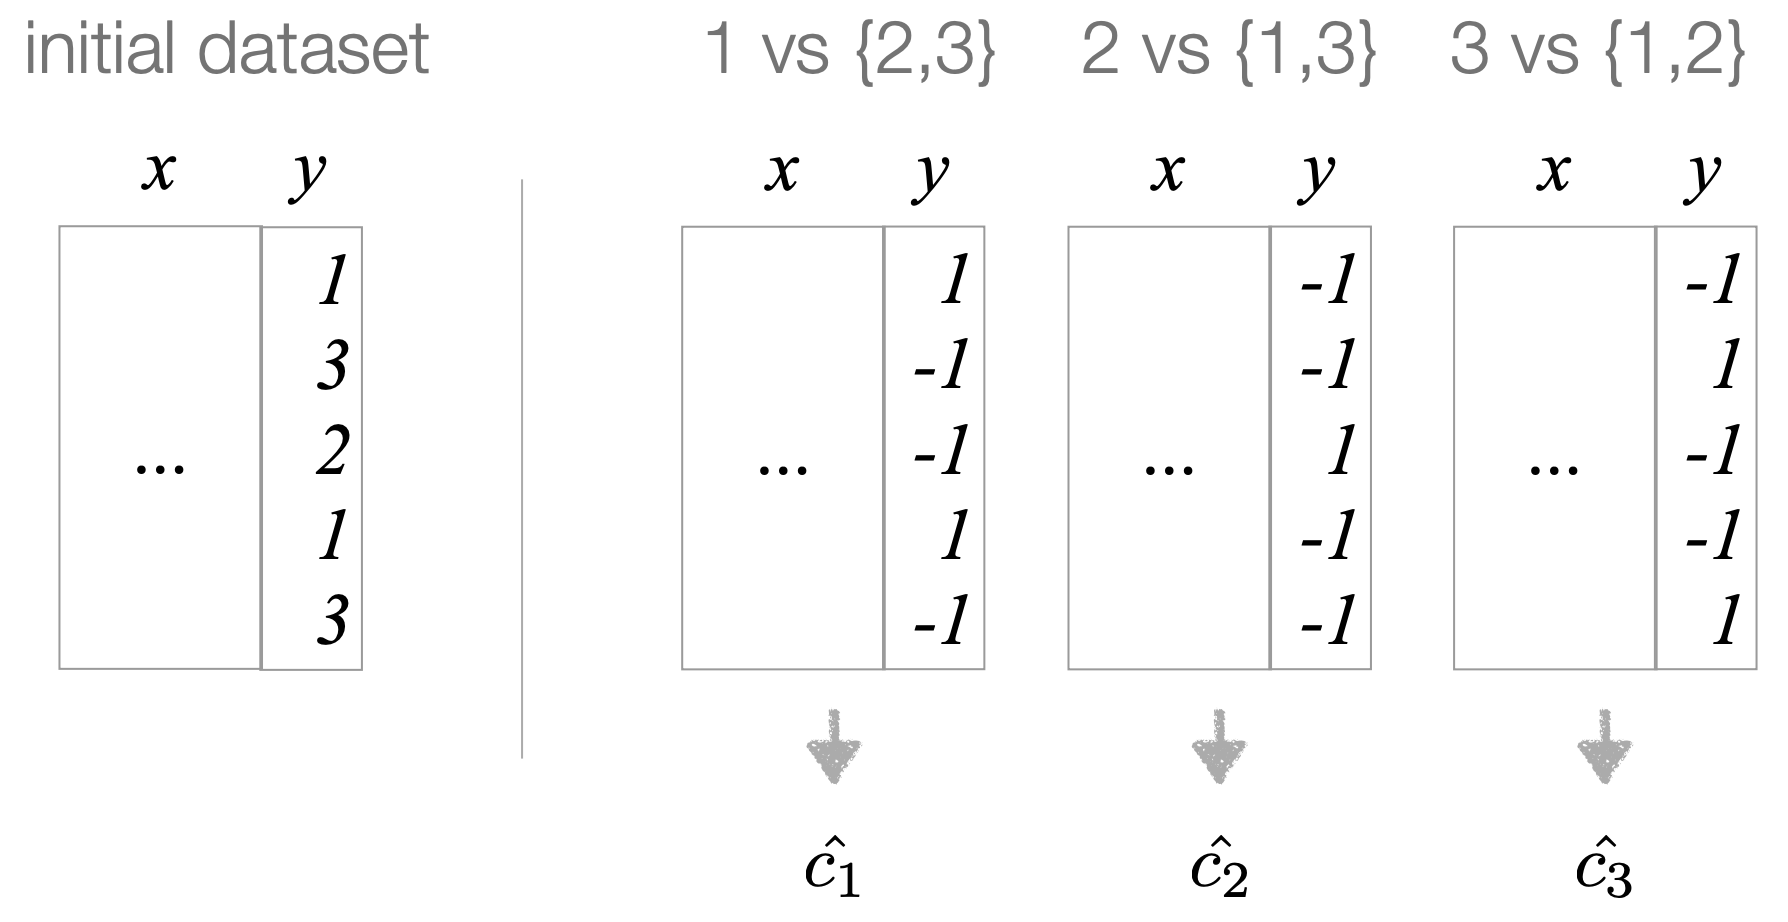
\includegraphics[scale=0.5]{images/unordered1vAll.png}
\end{figure}


L'idea è quella di costruire la prima volta un dataset che cerca di distinguere la classe 1 dalla 2 e 3, poi un secondo che distingue la 2 dalla 1 e 3 e infine un terzo che distingue la 3 dalla 1 e 2. Facciamo questa operazione prendendo il dataset iniziale e ovunque ci sia scritto 1 restituiamo in output 1, altrimenti -1. Applichiamo poi il nostro algoritmo di apprendimento $L$ al dataset per ottenere il classificatore $h_1$ e procediamo poi con gli altri due dataset ottenendo $h_2$ e $h_3$. A questo punto possiamo passare alla predizione, quindi arriva un nuovo esempio $x$ e bisogna classificarlo correttamente. Questo si fa semplicemente passando il parametro a tutti e 3 i classificatori e ottenendo un vettore con le predizioni (es: $X\xrightarrow{h_1,h_2,h_3}=(1,-1,-1)$). A questo punto è facile da tradurre in una classificazione n-aria.

Questo processo si può formalizzare con una matrice fatta in questo modo:
\begin{figure}[!h]
    \centering
    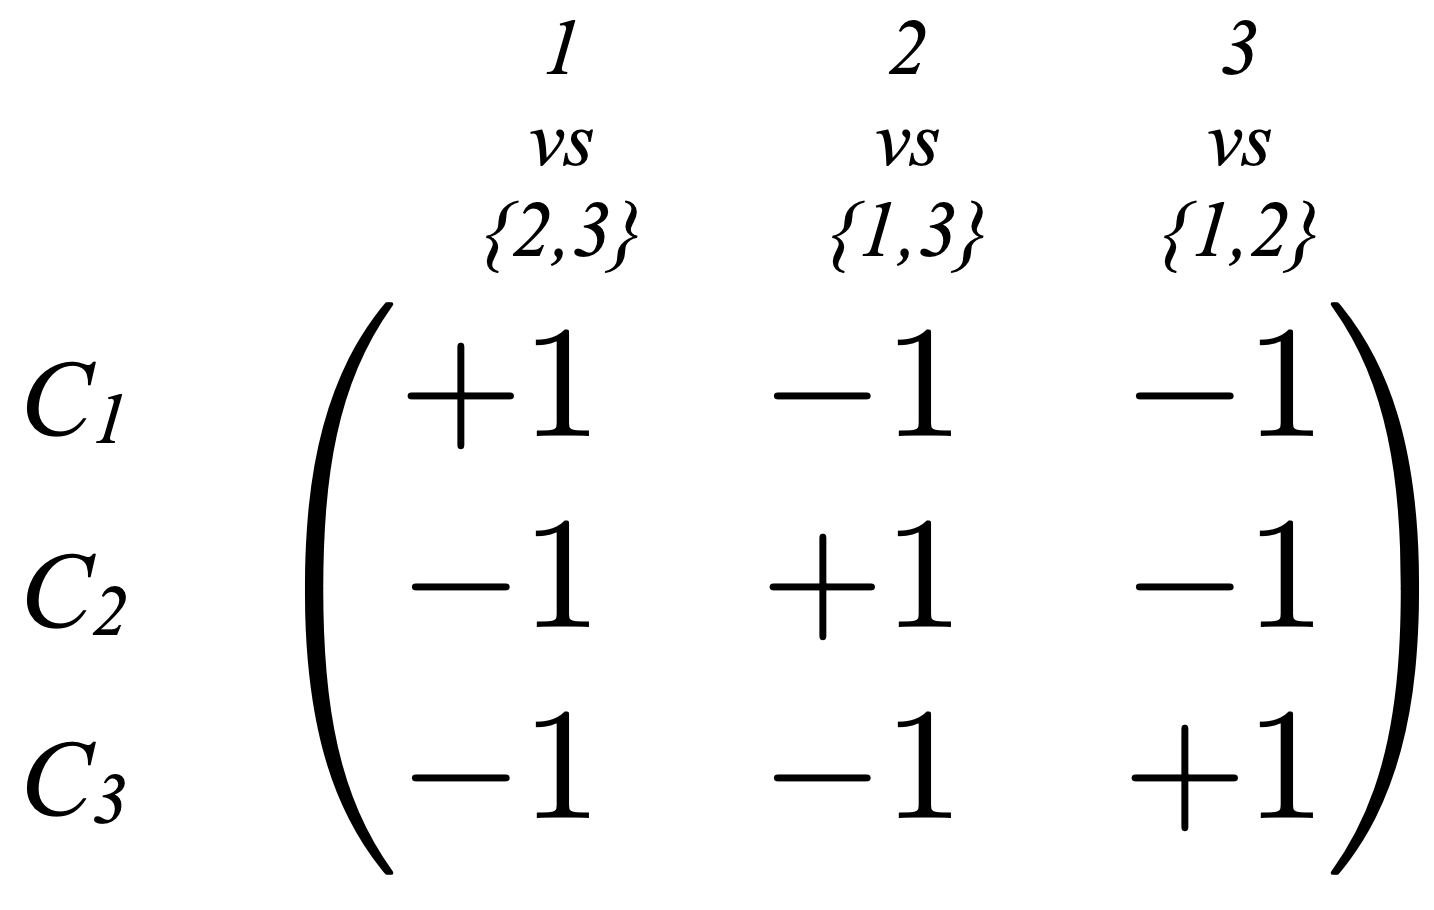
\includegraphics[scale=0.4]{images/matrixDisord.png}
\end{figure}


Questa matrice è utile sia nel momento della codifica che in quello della decodifica: nel momento della codifica le colonne ci dicono come fare il cambio delle etichette perchè, per esempio, la colonna 1 ci dice che, per il classificatore $1vs\{2,3\}$ , l'etichetta $c_1$ deve essere rinominata +1 e le altre -1.
Nel momento della decodifica, andiamo a confrontare il vettore che ci arriva con le righe della matrice e la classe da assegnare al vettore è quella che corrisponde alla riga più vicina al vettore stesso.
Da questa matrice si possono definire le altre per gli altri schemi.
\newpage

\paragraph{Uno contro tutti (ordinato)}
\begin{center}
    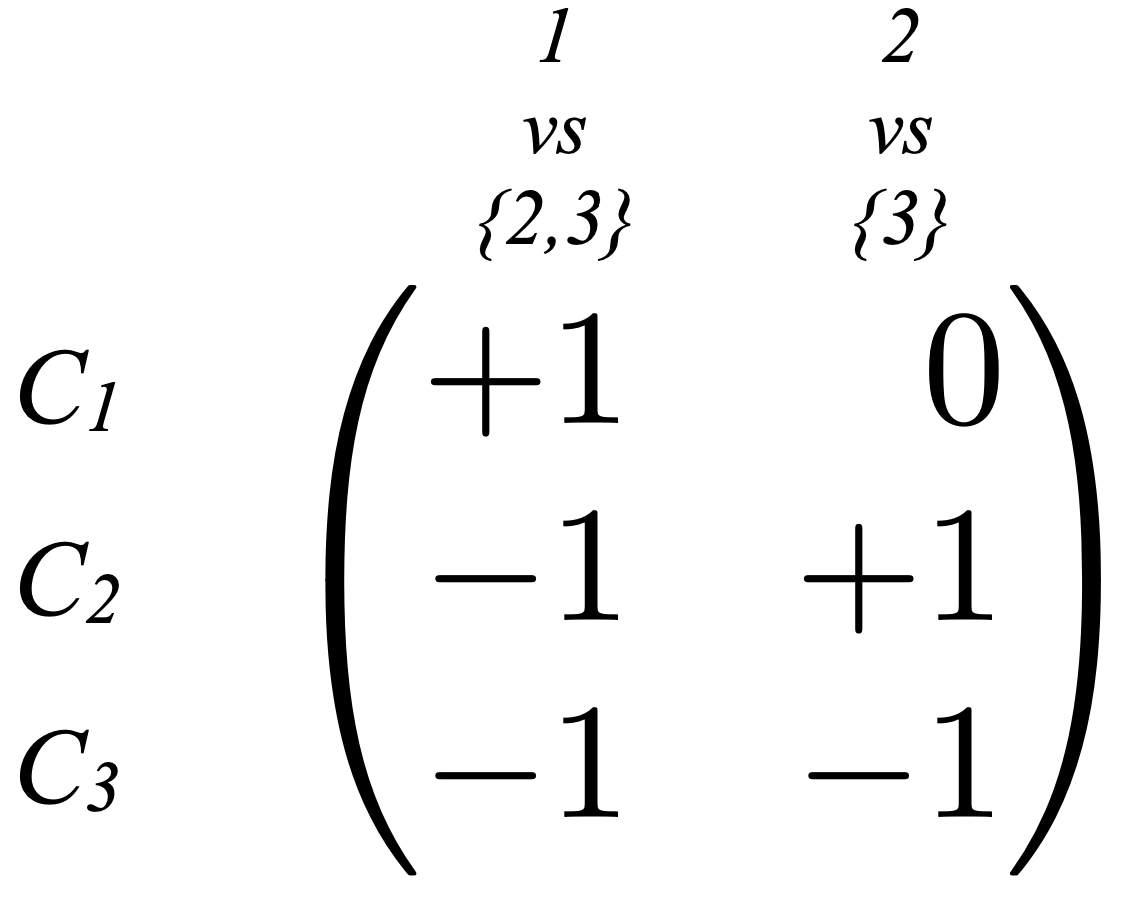
\includegraphics[scale=0.4]{images/matrixOrd.png}    
\end{center}

La differenza rispetto allo schema precedente sta nel fatto che qua consideriamo gli output dei classificatori in sequenza, quindi appena trovo un 1 mi fermo. Quindi non valuto tutti i classificatori.

\paragraph{Uno contro uno (simmetrico)}
\begin{center}
    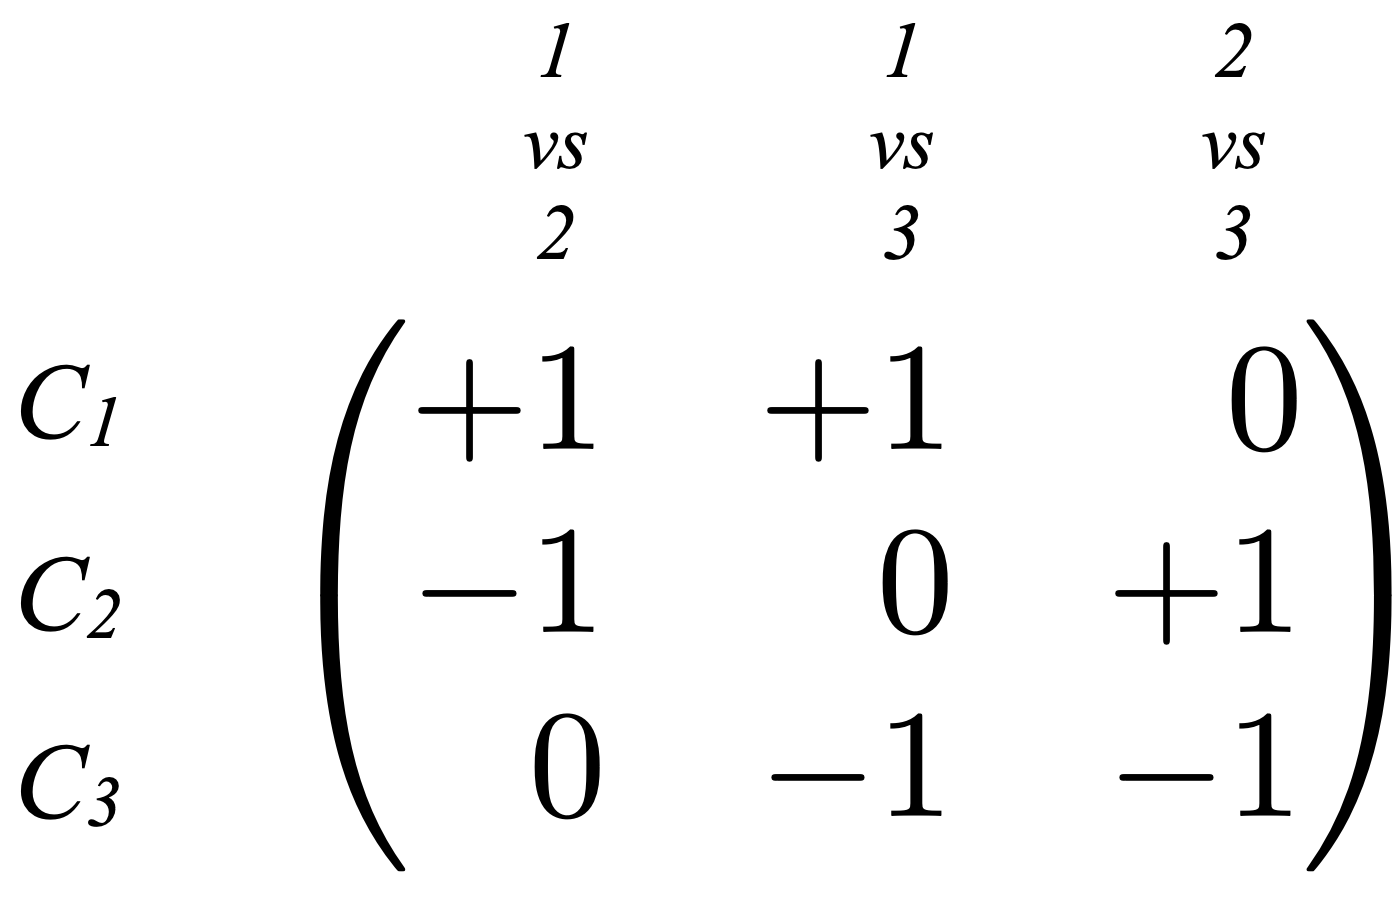
\includegraphics[scale=0.4]{images/matrixSymm.png}    
\end{center}

Qui l'idea è che al posto di creare un classificatore che confronta ogni classe con tutte le altre, creo un classificatore per ogni possibile coppia. Si mette 0 quando il modello si astiene.

\paragraph{Uno contro uno (asimmetrico)}
\begin{center}
    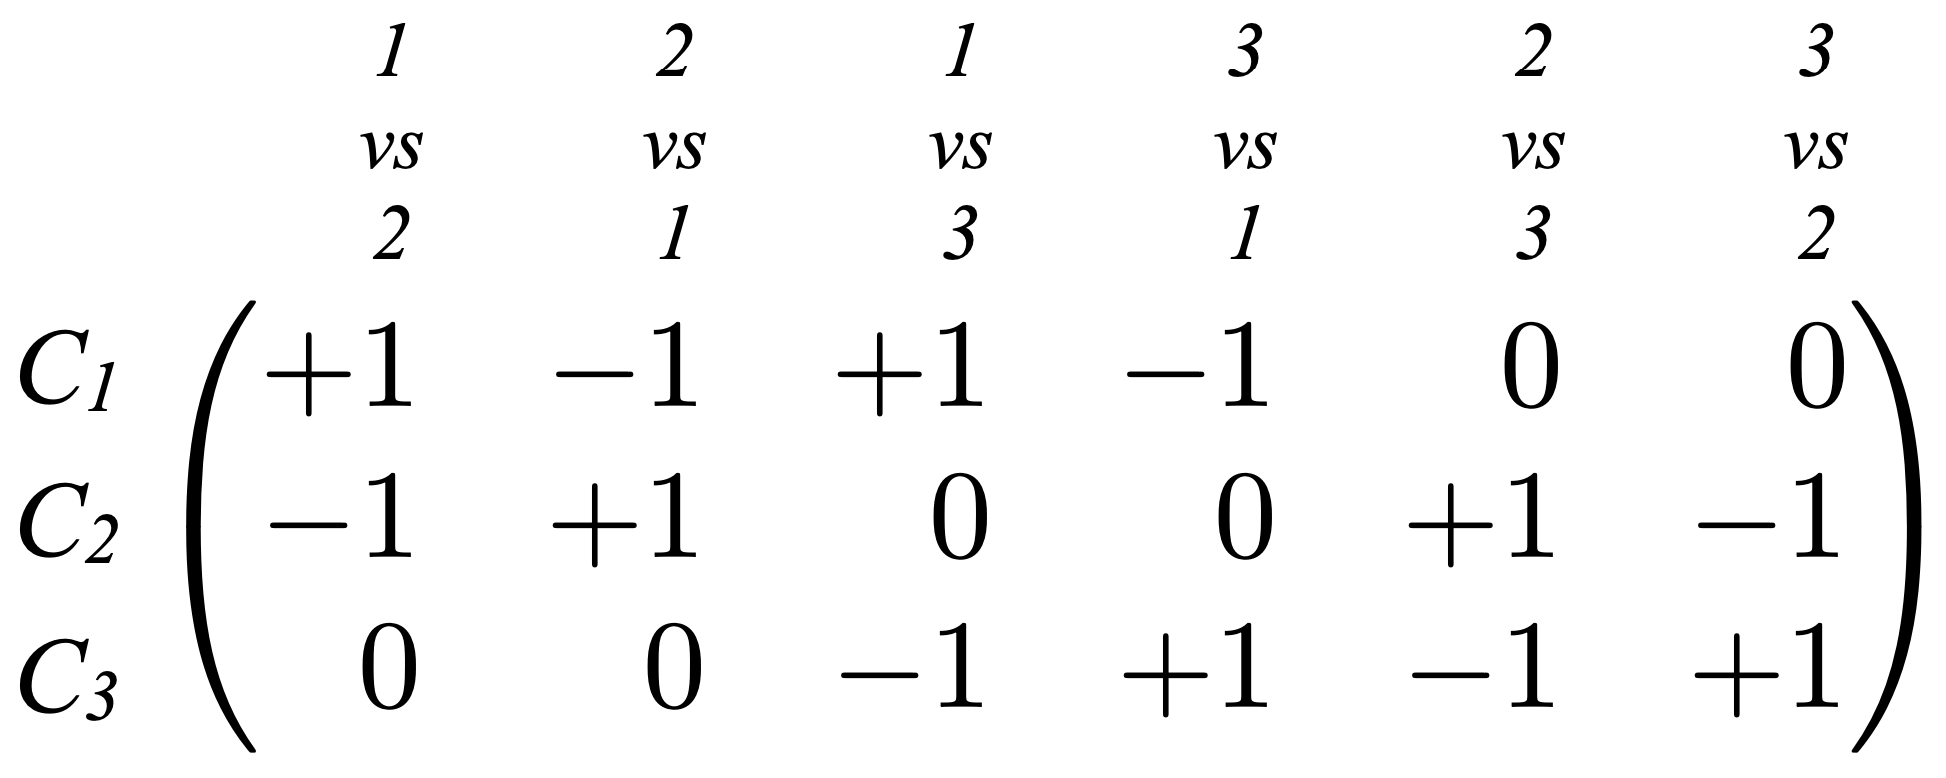
\includegraphics[scale=0.4]{images/matrixAsymm.png}    
\end{center}

L'unica differenza con il precedente sta nel fatto che si considerano anche tutte le coppie inverse (quindi sia $1vs2$ che $2vs1$).

\newpage

\paragraph{Decoding.} Nel caso di uno vs tutti (non ordinato) abbiamo detto che confrontiamo la distanza tra il vettore in input e le righe della matrice, ma come si calcola questa distanza? Così:
\begin{equation}
    d(w,c)=\frac{\sum_i(1-c_iw_i)}{2}
\end{equation}
in cui $w$ è il vettore che contiene gli output dei classificatori binari e $d$ è effettivamente la distanza. Se la classificazione è binaria $c_iw_i$ è 1 se sto classificando correttamente, -1 altrimenti.
\textbf{Esempio}:
\begin{center}
    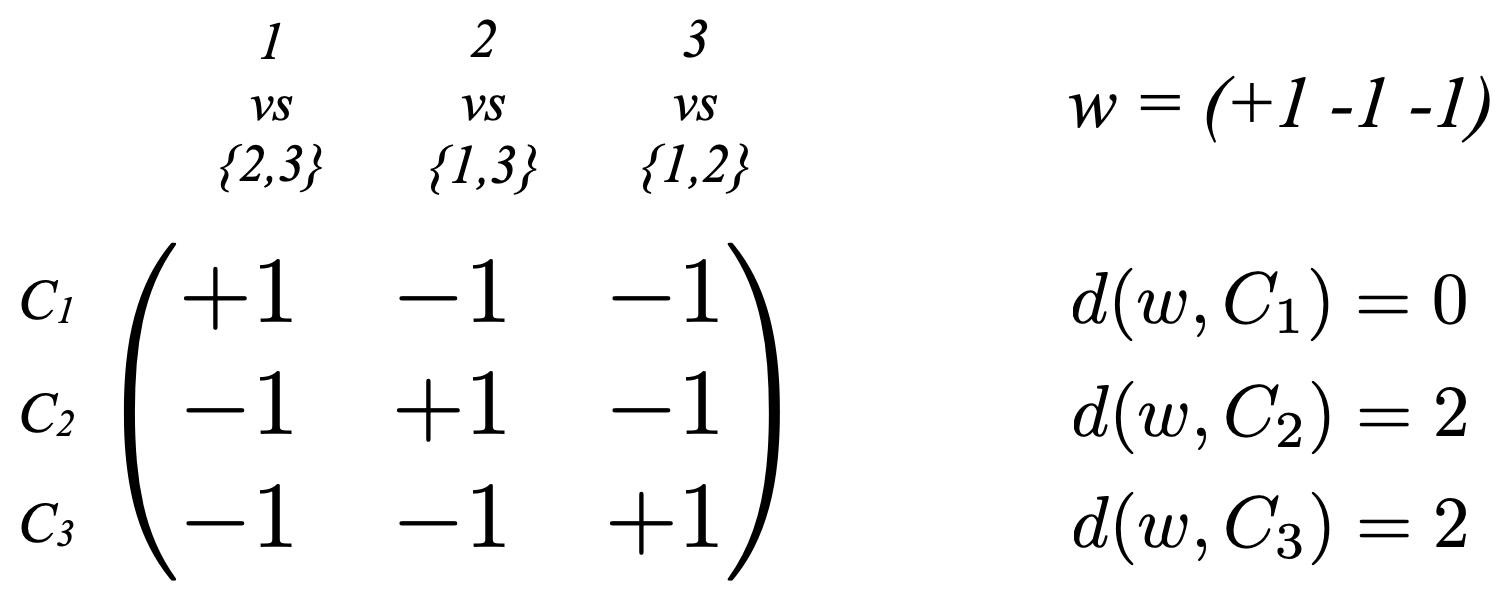
\includegraphics[scale=0.4]{images/matrixRis.png}    
\end{center}

Cosa succede se per esempio $w=(+1,-1,+1)$? Nel caso di $c_1$ abbiamo $d=1$, per $c_2$ abbiamo $d=3$ e per $c_3$ abbiamo di nuovo $d=1$. Siamo in un caso di ambiguità, come scelgo? Possiamo fare diverse cose: la più banale è prendere a caso uno dei due; un altra soluzione è vedere se questo è un problema diffuso nel dataset e quindi aggiungere colonne così da rendere questo caso ambiguo, più difficile da capitare. Un altro approccio è quello di usare un modello che dia uno score o uno probabilistico.

\paragraph{Difficoltà nell'applicare gli schemi.} Non usiamo sempre lo stesso schema perchè non ce n'è uno migliore dell'altro, entrambi hanno i loro vantaggi e i loro svantaggi. 

In particolare gli\textbf{uno vs tutti} si usano con un dataset non bilanciati, ovvero che non hanno circa lo stesso numero di esempi positivi e negativi.


Gli \textbf{uno contro uno} cercano di mitigare il problema assegnando l'etichetta 0 agli esempi che non appartengono alle 2 etichette prese in consederazione. Questo risulta particolarmente problematico quando il dataset è scarso di esempi.


%minuto 43:28 lezione 4